\documentclass[conference]{IEEEtran}
\usepackage{amsmath,amssymb}
\usepackage{booktabs}
\usepackage{graphicx}
\usepackage[hidelinks]{hyperref}
\DeclareMathOperator*{\argmax}{arg\,max}
\newcommand{\OEH}{\textsc{OEH}}
\newtheorem{theorem}{Theorem}
\newtheorem{proposition}{Proposition}

\begin{document}
\title{Difficulty-Aware Offline Reinforcement Learning: Pilot-Only Forecasting of Learner-Specific Data Requirements in Stochastic Tabular MDPs}
\author{\IEEEauthorblockN{Author names to be completed}
\IEEEauthorblockA{Affiliations and correspondence to be completed}}
\maketitle

\begin{abstract}
How much logged data will a given offline reinforcement-learning learner need before it succeeds reliably? We cast this as probabilistic forecasting: from a pilot log of a finite stochastic MDP, predict for a specified learner the first of six data budgets at which at least eight of ten independent seeds reach and keep 95\% of the optimal normalized return, with a right-censored class when none does. Offline Effective Horizon (OEH) simulates the actual learner on MDPs drawn from a posterior fitted to the pilot, adds planning-risk and cross-fitted pilot diagnostics, and joins a full and a robust head with a shift gate whose loss on every forecast is bounded; we also bound the regret of budget decisions by the forecast's Brier score. Developed on opened panels and frozen, OEH was evaluated in three pre-registered tests on 660 new MDPs from an internal generator and seven external sources (688,320 learner jobs). It beat the same forecasting procedure on generic pilot statistics in every final test (registered in Tests 1 and 3, descriptive in Test 2), by 37.7\% in integrated Brier score and 23.4\% in log loss on 228 external MDPs, and on a final test registered on the budgets beyond the pilot it beat a calibrated baseline that trains the learner on pilot prefixes and scores it by fitted Q evaluation, by 25.6\% and 17.9\%. Its advantage over the strongest pilot-only control and the benefit of the gate were panel-dependent, and a tabular foundation model on generic statistics matched OEH inside the generator but not outside it.
\end{abstract}
\begin{IEEEkeywords}
offline reinforcement learning, data requirement forecasting, right censoring, posterior predictive simulation, pre-registered evaluation
\end{IEEEkeywords}

\section{Introduction}
\label{sec:intro}

An offline reinforcement-learning (RL) learner must act from a fixed log; it cannot gather new evidence while it trains~\cite{levine2020offline}. A practitioner who holds a small pilot log therefore faces a planning question before committing to a large collection or training grid: \emph{how much logged data will this learner need before it reliably reaches a target return?} Dataset size alone does not answer it. Two logs of equal size can differ in which state--action pairs they cover, in the quality of the logging behavior and in how much transition noise must be averaged out, and the answer depends on the learner: behavior cloning (BC) cannot exceed a poor behavior, whereas a value-based learner can improve on it if the relevant actions are logged~\cite{kumar2022prefer}.

Three obvious shortcuts are insufficient. Dataset-quality scores~\cite{schweighofer2022dataset,swazinna2021quality,asadulaev2026bwd} summarize a log in one number that is not tied to a learner or a budget. Sample-complexity bounds~\cite{li2024sample,wang2022gapoffline} are worst-case or depend on unknown instance quantities. Training the learner on prefixes of the pilot and extrapolating its learning curve~\cite{domhan2015speeding,adriaensen2023efficient} sees only budgets smaller than the pilot, and its success must itself be estimated off-policy~\cite{le2019batch,voloshin2021empirical}. We did not find, in a scoped search, a method whose output is the \emph{distribution of the first data budget at which a specified offline learner attains sustained success}, estimated from a pilot and scored against censored outcomes.

We study this task in finite stochastic Markov decision processes (MDPs), where every policy can be evaluated exactly, so the target is measured rather than estimated. A forecaster sees one pilot of $10|S||A|$ transitions and public metadata; for BC, conservative fitted Q-iteration (CFQI) or tabular implicit Q-learning (IQL)~\cite{kostrikov2022iql} it outputs seven probabilities over the budgets $x1,\ldots,x50$ (multiples of $|S||A|$) and a right-censored class $>x50$. Our contributions are:
\begin{enumerate}
\item \textbf{Target and benchmark.} A learner-specific, right-censored requirement with a sustained-success rule, and a pipeline that generates controlled MDP families and converts MDPs and behaviors from eight external sources, seven of which enter the final tests, with exact evaluation.
\item \textbf{Method and guarantees.} Offline Effective Horizon (\OEH{}), which simulates the actual learner on MDPs drawn from a posterior fitted to the pilot, adds a planning-risk descriptor and cross-fitted pilot diagnostics, and joins a full and a robust head with a shift gate. We prove that the gate's loss on every forecast is bounded by its components' losses and that the regret of budget decisions is bounded by the forecast's integrated Brier score.
\item \textbf{Pre-registered evaluation.} \OEH{} was developed on opened panels only, frozen, and tested in three protocols on 660 new MDPs (688{,}320 learner jobs), each committed before its data existed, with an architecture-matched control, fixed-sequence gates and MDP-clustered simultaneous bounds. The last protocol registers an endpoint restricted to the budgets the pilot cannot reach and a baseline that trains the learner on pilot prefixes and scores it by fitted Q evaluation (FQE).
\end{enumerate}
\OEH{} beat generic pilot statistics in every final test (registered in Tests 1 and 3, descriptive in Test 2) and the pilot-extrapolation baseline on the extrapolation endpoint. We also report what did not hold: the advantage over the strongest pilot-only control and the benefit of the gate were panel-dependent, and a tabular foundation model on generic statistics matched \OEH{} inside the generator.

\section{Related Work}
\label{sec:related}

\textbf{Dataset characterization.} Trajectory quality and state--action coverage relate offline datasets to learner performance~\cite{schweighofer2022dataset}; ERI~\cite{swazinna2021quality} and the Bellman--Wasserstein distance~\cite{asadulaev2026bwd} score dataset quality, and image representations of a dataset predict the return of a learner trained on it~\cite{mateos2024images}. These methods output a score or a return at one configuration, some with reference data from the true environment. We use ERI and BWD as adapted input features under our head and the author-code TQ/SACo as a privileged comparison.

\textbf{Offline sample complexity and the effective horizon.} Coverage of the relevant policy and action gaps governs offline sample complexity~\cite{rashidinejad2021bridging,li2024sample,wang2022gapoffline}. The effective horizon links the lookahead depth at which greedy actions become correct to the effort of interactive RL~\cite{laidlaw2023effective,laidlaw2024stochastic}. Our planning-risk descriptor keeps its depth-and-gap structure but replaces the true MDP by a posterior and random rollouts by the logging behavior, which voids the guarantees; we treat it as a feature to be validated.

\textbf{Learning curves and off-policy evaluation.} Learning-curve extrapolation predicts final performance from partial training runs, parametrically~\cite{domhan2015speeding} or with prior-data fitted networks~\cite{adriaensen2023efficient}; learning curves can be non-monotone~\cite{viering2023shape}, which motivates our sustained-success rule. Fitted Q evaluation estimates a policy's value from logged data~\cite{le2019batch,voloshin2021empirical}, and offline policy selection ranks trained policies~\cite{yang2022selection,tang2021selection}. Our strongest baseline combines both: it trains the learner on pilot prefixes, scores it by FQE on held-out folds and extrapolates.

\textbf{Censored forecasting and tabular models.} Right-censored outcomes are commonly modeled with accelerated failure time models~\cite{barnwal2022aft} or discrete-time classifiers~\cite{kim2026survival}; proper scores~\cite{gneiting2007strictly} evaluate the forecasts. Tabular foundation models such as TabPFN~\cite{hollmann2025accurate} predict in context without fitting; we use TabPFN v2 as a strong generic learner on the pilot statistics. Reusing validation data biases evaluation~\cite{cawley2010selection,dwork2015adaptive}, which is why development and final panels are kept apart.

\section{Problem Formulation}
\label{sec:problem}

\textbf{Setting.} Let $M=(\mathcal S,\mathcal A,P,R,\gamma,\rho)$ be a finite discounted MDP with $S$ states, $A$ actions and $\gamma=0.95$. A behavior policy $\beta$ generates a pilot log $D_0$ of $N_0=10SA$ transitions in episodes of at most 100 steps. An offline \emph{learner} $l$ maps a buffer to a policy. A \emph{forecaster} maps $(D_0,l)$, public metadata ($S$, $A$, $\rho$, $\gamma$) and a model fitted on earlier \emph{meta-training} cohorts to seven probabilities $p_{l,0},\ldots,p_{l,6}$. It never sees the true MDP. Fig.~\ref{fig:pipeline} separates the forecast and label paths.

\begin{figure*}[t]
\centering
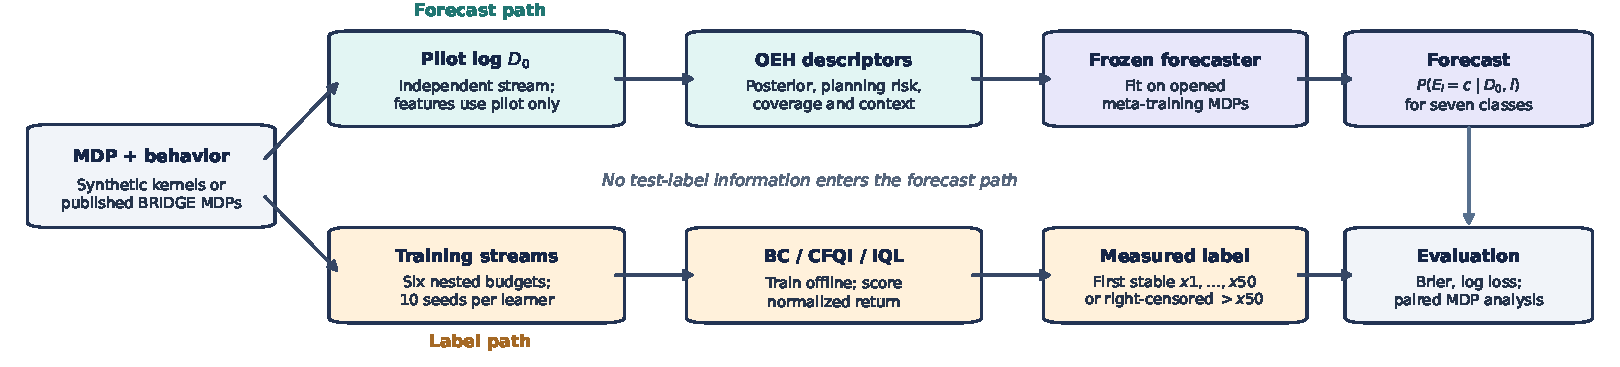
\includegraphics[width=\textwidth]{figures/oeh_pipeline.pdf}
\caption{Forecast path and label path. The pilot $D_0$ and learner identity enter the frozen forecaster; independent training streams at nested budgets and ten seeds per learner produce the measured, possibly censored requirement label. Forecasts are sealed before labels and joined only for scoring.}
\label{fig:pipeline}
\end{figure*}

\textbf{Learner-specific empirical requirement.} For a policy $\pi$ with value $J(\pi)=\rho^\top V^\pi$, the normalized return is
\begin{equation}
\mathrm{NR}(\pi)=\frac{J(\pi)-J_{\rm random}}{J^*-J_{\rm random}},
\label{eq:nr}
\end{equation}
computed exactly in the true MDP. A training seed succeeds when $\mathrm{NR}\geq\tau=0.95$. The budgets are $N_j=b_jSA$ with $b=(1,2,5,10,20,50)$, nested prefixes of each of ten independent training streams. With $\pi_{l,j,i}$ the policy of seed $i$ at budget $j$,
\begin{equation}
\begin{aligned}
C_{l,j}&=\textstyle\sum_{i=1}^{10}\mathbf 1\{\mathrm{NR}(\pi_{l,j,i})\geq\tau\},\\
E_l&=\min\bigl\{j:\min\nolimits_{m\geq j}C_{l,m}\geq 8\bigr\},
\end{aligned}
\label{eq:event}
\end{equation}
with $E_l=6$ ($>x50$) when no index qualifies. The suffix condition handles non-monotone learning curves: counts $(2,5,8,7,9,10)$ give $E_l=4$ ($x20$), not $x5$, because success at $x5$ is not sustained at $x10$. Class 6 is right censoring beyond the measured grid. The requirement is conditional on MDP, behavior, learner, threshold and protocol; it is not an intrinsic property of $M$. Because the pilot already costs $x10$, the classes $x1$--$x5$ are retrospective; Section~\ref{sec:method} defines an endpoint restricted to the budgets beyond the pilot.

\textbf{Information access.} The pilot and training streams use disjoint seed namespaces, and the true kernel is used only to generate data and to score policies. No pilot-only statistic can identify the value of an action that was never logged: two MDPs that agree on every logged action produce the same pilot distribution. Our posterior therefore encodes a convention (unobserved reward keys receive zero), not a certificate. Comparators that use the true MDP or reference data from it are labeled \emph{privileged}.

\section{Offline Effective Horizon}
\label{sec:method}

\OEH{} turns a pilot into a seven-class forecast in four stages: a Bayesian model of the MDP and the behavior is fitted to the pilot counts; signals are derived from this posterior and from the pilot; three fitted predictors map them to class probabilities; and a shift gate combines the predictors according to how far the pilot lies from the meta-training data.

\textbf{Posterior-predictive learner simulation (OEH-B).} Pilot counts update Dirichlet models of the transition rows (uniform base, concentration by marginal likelihood) and of the behavior (a Dirichlet mixture). Observed reward keys keep their logged values and unobserved keys receive zero. For each of $B=64$ posterior draws, OEH-B simulates ten nested streams up to $x50$, trains the \emph{same} registered learner on the six prefixes, evaluates the policies exactly in the drawn MDP and applies Eq.~\eqref{eq:event}. With $B_{\rm eff}$ draws that pass the dynamic-range condition of the benchmark, the smoothed law is the Krichevsky--Trofimov estimate~\cite{krichevsky1981encoding}
\begin{equation}
\widehat p^{\,\rm B}_l(c)=\frac{\#\{b:E_l^{(b)}=c\}+\tfrac12}{B_{\rm eff}+\tfrac72},\qquad c=0,\ldots,6.
\label{eq:posterior}
\end{equation}
OEH-B also records the simulated success rate and normalized return at each budget. Under coverage, concentration and genericity assumptions the idealized raw law converges to the true requirement law (supplement), but at $x10$ it is far from that regime and is poorly calibrated on its own, so it is an input to the fitted heads.

\textbf{Planning-risk descriptor (OEH-H).} On the posterior-mean model, OEH-H starts from $Q_1=Q^{\bar\beta}$ and applies Bellman backups restricted to the modeled support. At depth $k$, with $\pi_k$ greedy, $\Delta_k(s,a)$ the backed-up gap to a competitor $a$, $L_k(s,a)$ its loss under $Q^{\pi_k}$ and $d^{\pi_k}_\rho$ the normalized discounted occupancy, the modeled regret at $N$ logged transitions is
\begin{equation}
\begin{aligned}
w_k(s,a)&=\frac{d^{\pi_k}_\rho(s)\,L_k(s,a)}{(1-\gamma)(J^*-J_{\rm random})},\\
\widetilde\ell_k(N)&=\sum_{s,a}w_k(s,a)\,
\Phi\!\left(\frac{-\Delta_k(s,a)\sqrt N}{\sqrt{\nu_k(s,\pi_k(s))+\nu_k(s,a)}}\right),
\end{aligned}
\label{eq:risk}
\end{equation}
where $\nu_k$ propagates the Bellman-target variance divided by the logging visitation to first order, and the weighting follows the performance-difference identity~\cite{kakade2002approximately}. Inverting the risk against the return slack gives
\begin{equation}
h_{\rm H}=\min_{k:\,\mathrm{NR}(\pi_k)\ge\tau}\log_A\inf\{N\ge1:\widetilde\ell_k(N)\le\mathrm{NR}(\pi_k)-\tau\},
\label{eq:oehh}
\end{equation}
over depths 1--100. OEH-H also reports the risk and an exponential missing-mass estimate at each budget, the return ceilings of the posterior-mean behavior and of the \emph{observed} support, and concentrability summaries. Eqs.~\eqref{eq:risk}--\eqref{eq:oehh} are descriptors, not finite-sample bounds.

\textbf{Pilot diagnostics (D).} Two diagnostics read the pilot directly. An action-identification risk multiplies the performance-difference impact of confusing each supported top/runner-up pair by an empirical-Bernstein error tail~\cite{maurer2009empirical} and inverts it into a requirement. A cross-fit trains the actual learner on four of five hash-assigned trajectory folds at the nested pilot prefixes $x2$, $x5$, $x10$ and evaluates it in a pessimistically completed model of the held-out fold; the risk at three prefixes gives a contraction rate.

\textbf{Features and predictors.} The 108 columns form eight lineage blocks: B2 generic statistics (G1, 18: size, coverage, entropy, return, bootstrap spread), OEH-B summaries of the row's learner (G2, 18), posterior concentrations (G3, 2), OEH-H descriptors (G4, 11) and risk profile (G5, 13), OEH-B laws of all three learners (G6, 18), and the diagnostics D of the row (G7, 10) and of all learners (G8, 18). A \emph{matched head} has three components fitted per learner: an XGBoost accelerated-failure-time model~\cite{barnwal2022aft} on the interval-censored budget, six monotone-projected threshold classifiers for $P(E_l\le j)$, and a multiclass model; convex weights minimize out-of-fold log loss over five MDP-grouped folds. \OEH{} fits three predictors with it: the \emph{full head} (OEH-F) on all 108 columns, a finite-only full head on the rows with $E_l<6$, and the \emph{robust head} on B2 + D (46 columns). Every matched comparator uses the identical procedure with its own features.

\textbf{Scores.} With $F_{l,j}=\sum_{c\le j}p_{l,c}$, the registered scores are
\begin{equation}
\begin{aligned}
\mathrm{IBS}&=\tfrac16\textstyle\sum_{j=0}^{5}\bigl(F_{l,j}-\mathbf 1\{E_l\le j\}\bigr)^2,\\
\mathrm{LL}&=-\log\max(p_{l,E_l},10^{-12}),
\end{aligned}
\label{eq:scores}
\end{equation}
both proper and lower-is-better~\cite{gneiting2007strictly}; a censored row contributes six zero targets to the IBS and $p_{l,6}$ to the LL. The \emph{extrapolation endpoint} keeps only budgets the pilot cannot reach:
\begin{equation}
\begin{aligned}
\mathrm{IBS}_{\ge}&=\tfrac13\textstyle\sum_{j=3}^{5}\bigl(F_{l,j}-\mathbf 1\{E_l\le j\}\bigr)^2,\\
\mathrm{LL}_{\rm ext}&=-\log\max(\tilde p_{l,\tilde E_l},10^{-12}),
\end{aligned}
\label{eq:ext}
\end{equation}
where $\tilde p_l$ coarsens the forecast to $\{\le x10, x20, x50, >x50\}$.

\subsection{Shift gate}
\label{sec:v2}
On development panels from other groups' procedures, the full head kept recognizing insufficient data but placed finite requirements worse than simpler forecasters (Section~\ref{sec:development}). The gate therefore keeps the full head's censored probability $p_6$ and moves the finite part toward the robust head as the pilot leaves the training distribution. Let $d$ be the mean distance of the pilot's standardized B2 statistics to its ten nearest meta-training rows, $\lambda(d)=\lambda_{\max}\min(1,d/d_0)$ and $\varepsilon(d)=\varepsilon_{\max}\min(1,d/d_0)$. With $q_O$ the law of the finite-only full head, $q_R$ the renormalized finite part of the robust head and $\bar p_l$ the learner's meta-training class frequencies,
\begin{equation}
p^{\OEH}=(1-\varepsilon)\bigl[(1-p_6)\bigl((1-\lambda)q_O+\lambda q_R\bigr),\;p_6\bigr]+\varepsilon\,\bar p_l .
\label{eq:v2}
\end{equation}
The options for $q_O$ and $q_R$ and $(\lambda_{\max},\varepsilon_{\max},d_0)$ were chosen on opened development panels by a rule written before any fit (Section~\ref{sec:setup}): $\lambda_{\max}=1$, $\varepsilon_{\max}=0.02$, $d_0=3$.

\subsection{Guarantees}
\label{sec:theory}
Both bracketed forecasters in Eq.~\eqref{eq:v2} share $p_6$, so $p^{\OEH}$ is a mixture of three complete forecasters with weights that depend only on $d$.

\begin{proposition}[Per-forecast bound]
\label{prop:gate}
For every pilot and outcome $y$, under any shift, the IBS and the LL of $p^{\OEH}$ are at most the $d$-weighted average of its three components' scores; $-\log p^{\OEH}_y\le-\log(\varepsilon(d)\bar p_{l,y})$; and on a censored row the LL exceeds that of the full head by at most $-\log(1-\varepsilon_{\max})\le0.0203$ nat.
\end{proposition}
\noindent Both scores are convex in the probability vector, so the bound is Jensen's inequality (supplement). It limits what the gate can lose; it does not say that the gate helps.

Forecasts are meant to drive budget decisions. Suppose a practitioner collects budget $b_a$ and trains, paying $b_a$ plus a penalty $\kappa$ if $E_l>a$, or skips, paying $\kappa$ if $E_l\le5$. For a cumulative forecast $F$ the expected costs are $C(a;F)=b_a+\kappa(1-F_a)$ and $C(\mathrm{skip};F)=\kappa F_5$, and $a(F)$ minimizes them. Let $F^\star=\Pr(E_l\le\cdot\mid\mathcal G)$ for an information set $\mathcal G$ to which $F$ is measurable.

\begin{theorem}[Regret from scoring]
\label{thm:regret}
On every row, $C(a(F);F^\star)-C(a(F^\star);F^\star)\le2\kappa\max_j|F_j-F^\star_j|$, and in expectation the regret is at most $2\kappa\sqrt{6\,\Delta}$, where $\Delta$ is the excess IBS of $F$ over $F^\star$.
\end{theorem}
\noindent\emph{Proof sketch.} Each cost differs between $F$ and $F^\star$ by at most $\kappa\|F-F^\star\|_\infty$, and $a(F)$ minimizes $C(\cdot;F)$, which gives the row bound. The cross term of the Brier decomposition vanishes by conditioning on $\mathcal G$, so $\mathbb E\|F-F^\star\|_2^2=6\Delta$; Jensen's inequality completes the proof. The supplement proves variants for the registered threshold rule (a margin bound) and for the excess log loss ($\kappa\sqrt{2\Delta_{\rm LL}}$, via Pinsker's inequality). The bounds hold on all final panels but are loose (Section~\ref{sec:cost}); they link the \emph{ordering} of probabilistic scores to the ordering of decision regret.

\textbf{What is not claimed.} The fitted trees are locally constant, so if the features converge off every split threshold the heads' outputs become constant. Two B2 statistics grow without bound with the pilot, however, so $d\to\infty$ and the gate saturates at the robust head's finite law. \OEH{} is therefore \emph{not} a consistent estimator of the requirement law; its limit is the heads' output at the boundary of the training range (supplement).


\section{Experimental Setup}
\label{sec:setup}

\textbf{Panels.} The target needs, for one MDP and behavior, an independent pilot, nested budgets, ten training seeds per learner and exact optimal and random returns. Published offline datasets do not supply this, so every panel is generated by one pipeline that replaces only the source of the MDP (and, for SPIBB, of the behavior). The internal generator draws stochastic Garnet, forward-layered and bottleneck MDPs ($32\le SA\le256$); each MDP has five behavior policies and passes an ex-ante return-span filter. External MDPs come from the Colosseum sampler~\cite{conserva2022hardness}, SPIBB's code and baseline behaviors~\cite{laroche2019spibb}, MDPToolbox forest management~\cite{chades2014mdptoolbox}, Gymnasium FrozenLake~\cite{towers2024gymnasium}, the gambler's problem~\cite{sutton2018reinforcement}, MDP Playground~\cite{rajan2023mdp} and DeepMind Lab's labmaze layouts~\cite{beattie2016deepmind}; episodic tasks restart from the initial distribution, and rewards lie in $[0,1]$. Table~\ref{tab:setup} lists the panels by role: meta-training fits every head, development panels were opened while \OEH{} was built and are used for selection only, and final panels were generated after the method was frozen and evaluated once.

\begin{table}[t]
\centering
\caption{Panels by role (MDPs). $^{*}$MDP and logging behavior from the SPIBB authors' code. The final tests used 688{,}320 learner jobs.}
\label{tab:setup}
\footnotesize
\setlength{\tabcolsep}{2.5pt}
\begin{tabular}{@{}llr@{}}
\toprule
Role & Panel (source) & MDPs\\
\midrule
Meta-training & seven internal cohorts & 720\\
\midrule
Development & cohort 7 (sealed test of the full head) & 84\\
(opened) & cohort 8 (internal) & 168\\
 & Colosseum, sampler seeds 2027 and 2028 & 72 + 72\\
 & SPIBB$^{*}$ & 108\\
\midrule
Final test 1 & internal (new kernels) & 168\\
(four panels) & Colosseum, sampler seed 2029 & 72\\
 & SPIBB-2$^{*}$ (new seeds); forest management & 108; 48\\
Final test 2 & FrozenLake; gambler's problem & 36; 36\\
Final test 3 & MDP Playground; labmaze & 96; 96\\
\bottomrule
\end{tabular}
\end{table}

\textbf{Learners.} BC counts actions with a uniform fallback; CFQI performs up to 100 Bellman backups restricted to observed actions; IQL~\cite{kostrikov2022iql} uses expectile 0.7 and inverse temperature 3. Imitation, conservative value iteration and advantage-weighted extraction react differently to coverage and behavior quality. Final panels extend the training streams to $x200$; the primary label uses the first six budgets.

\textbf{Comparators.} All see the same pilot and meta-training panel. \emph{B2 matched} fits the identical head on the 18 generic statistics, so a gain cannot come from a stronger head or more labels. The \emph{robust head} (B2 + D) was the strongest pilot-only control in development. \emph{OEH-F} is the full head without the gate. \emph{LCE} extrapolates the learner's success curve on the nested pilot prefixes evaluated in posterior MDPs, and \emph{CB} uses offline concentrability quantities~\cite{li2024sample}; both are used alone and added to B2. \emph{Prefix + FQE}, specified in writing before its first run, trains the learner on prefixes of $1,2,4,8\times SA$ transitions of four pilot folds, scores each policy by tabular FQE~\cite{le2019batch} on the held-out fold, fits a monotone logistic curve in $\log b$ and maps it to the 8-of-10 rule; \emph{B2 + prefix/FQE} feeds its ten curve features to the matched head. \emph{XGBoost-CF} adapts a discrete-time survival classifier~\cite{kim2026survival}, \emph{TabPFN v2}~\cite{hollmann2025accurate} is run on B2 with default settings and no tuning, and a $k$-nearest-neighbor analog and a multinomial logistic regression on B2 are generic controls. Privileged comparators (oracle effective horizon, TQ/SACo with reference data~\cite{schweighofer2022dataset}) were evaluated in development only.

\textbf{Protocol and inference.} Scores are averaged over the rows of each MDP and then over MDPs, the independent unit. Simultaneous one-sided 95\% lower bounds (LB) resample whole MDPs 10{,}000 times with a max-$t$ rule at the original standard error; a contrast passes when its LB is positive. The gate was selected on the five development panels by a rule written before any fit: a grid over two head options, $\lambda_{\max}$, $\varepsilon_{\max}$ and $d_0$, minimizing mean external relative IBS and LL subject to both in-generator scores within $+2\%$ of OEH-F, and preferring the simplest candidate within 0.002. Three further changes (a single head, an exchangeable reward prior, three new behavior families in meta-training) failed rules written before they were tried. Each final protocol was committed and pushed before any data of its panels existed, and each panel's forecasts were sealed before its first learner job:
\emph{Test 1} is a fixed sequence: (1) \OEH{} vs the robust head on the pooled external MDPs; (2) non-inferiority to OEH-F inside the generator (2\% margin) and superiority outside; (3) superiority to B2, XGBoost-CF/18, LCE, CB, B2 + LCE and B2 + CB, inside and outside.
\emph{Test 2} registers one family, \OEH{} vs the robust head.
\emph{Test 3} registers, on $\mathrm{IBS}_\ge$ and $\mathrm{LL}_{\rm ext}$ (Eq.~\eqref{eq:ext}), F1: \OEH{} vs B2 + prefix/FQE, then F2: vs B2, and F3: the regret difference as an estimate without a verdict.
\OEH{} was built over earlier sealed tests of the forecasting question, three of which failed; each gate controls its error within its own test, and the program as a whole is adaptive.

\section{Results}
\label{sec:results}

\subsection{Test 1: four new panels}
\label{sec:v2test}
Table~\ref{tab:v2test} reports the first final test (371{,}520 learner jobs). All three steps pass. Against the robust head on the 228 pooled external MDPs, \OEH{} improves IBS by $0.0171$ (LB $+0.0107$) and LL by $0.0597$ ($+0.0344$). Inside the generator it is non-inferior to OEH-F (LB $+0.0003$ and $+0.0045$ on $1.02\cdot\text{OEH-F}-\OEH{}$; the forecasts nearly coincide, since the median $d$ is 1.1), and outside it beats OEH-F by $0.0047$ ($+0.0028$) and $0.0662$ ($+0.0398$). All 24 step-3 bounds are positive. Relative to B2 matched, \OEH{} lowers IBS and LL by 15.7\% and 8.3\% inside the generator and by 37.7\% and 23.4\% outside, with per-panel intervals excluding zero everywhere. The margin over the robust head, however, comes from forest management ($+0.070$ IBS, $+0.23$ LL); on Colosseum it is not individually significant ($+0.0074$ $[-0.0055,0.0204]$), on SPIBB-2 the methods tie, and without forest the pooled gain is $+0.0030$ $[-0.0022,0.0082]$. The only learner cells where \OEH{} is significantly worse than OEH-F are the all-censored BC and IQL rows of SPIBB-2, by at most 0.003 nat, within Proposition~\ref{prop:gate}.

\begin{table*}[t]
\centering
\caption{Test 1 (IBS / LL, MDP-averaged; lower is better; best in bold). Gate: step 1 vs the robust head on the pooled external MDPs, LB $+.0107$ / $+.0344$; step 2 non-inferiority to OEH-F inside (LB $+.0003$ / $+.0045$) and superiority outside (LB $+.0028$ / $+.0398$); step 3 all 24 contrasts positive.}
\label{tab:v2test}
\footnotesize
\setlength{\tabcolsep}{4pt}
\begin{tabular}{@{}lccccc@{}}
\toprule
Method & Internal (168) & Colosseum 2029 (72) & SPIBB-2 (108) & Forest (48) & Pooled external (228)\\
\midrule
\OEH{} & .0476 / \textbf{.562} & \textbf{.1080} / \textbf{.833} & .0189 / .358 & \textbf{.1097} / \textbf{.790} & \textbf{.0662} / \textbf{.599}\\
OEH-F (no gate) & \textbf{.0475} / .563 & .1153 / .951 & \textbf{.0188} / \textbf{.352} & .1216 / .941 & .0709 / .665\\
Robust head (B2 + D) & .0497 / .579 & .1154 / .873 & .0190 / .354 & .1794 / 1.022 & .0832 / .659\\
B2 + LCE & .0544 / .597 & .1396 / .995 & .0249 / .400 & .1299 / .865 & .0832 / .686\\
B2 matched & .0565 / .613 & .1407 / .989 & .0252 / .420 & .2370 / 1.285 & .1063 / .782\\
XGBoost-CF/18 & .0596 / 1.122 & .1436 / 1.256 & .0277 / .457 & .2535 / 1.447 & .1118 / .918\\
\bottomrule
\end{tabular}
\end{table*}

\subsection{Tests 2 and 3: four new sources}
\label{sec:fifth}
\textbf{Test 2} registered only the contrast with the robust head, on 72 MDPs from FrozenLake (slippery) and the gambler's problem. It is \textbf{NO-GO}: \OEH{} changes IBS by $-0.0017$ (LB $-0.0067$) and LL by $+0.0117$ ($-0.0196$). On FrozenLake every requirement is censored; \OEH{} recognizes this far better than the robust head ($+0.0065$ IBS, $+0.072$ LL), but the learner's own pilot learning curve (LCE) is better still. On the gambler's problem the robust head is better, mainly for BC. Descriptively, \OEH{} again beats OEH-F ($+0.0009$ IBS, $+0.020$ LL, intervals excluding zero) and B2 in LL ($+0.058$ $[0.031,0.086]$) (Table~\ref{tab:fifth}).

\begin{table}[t]
\centering
\caption{Test 2 (IBS / LL). Registered contrast \OEH{} vs robust head: NO-GO. All FrozenLake requirements are censored.}
\label{tab:fifth}
\footnotesize
\setlength{\tabcolsep}{3pt}
\begin{tabular}{@{}lccc@{}}
\toprule
Method & FrozenLake (36) & Gambler (36) & Pooled (72)\\
\midrule
\OEH{} & .0040 / .082 & .0931 / .752 & .0486 / \textbf{.417}\\
OEH-F (no gate) & .0038 / .079 & .0951 / .795 & .0495 / .437\\
Robust head (B2 + D) & .0105 / .154 & .0831 / \textbf{.703} & \textbf{.0468} / .428\\
B2 matched & .0122 / .153 & .0958 / .797 & .0540 / .475\\
LCE raw & \textbf{.0007} / \textbf{.025} & .1132 / 1.174 & .0569 / .599\\
$k$-NN analog on B2 & .0176 / .243 & \textbf{.0795} / .728 & .0486 / .485\\
\bottomrule
\end{tabular}
\end{table}

\textbf{Test 3} asks whether the advantage lies in the budgets the pilot cannot reach and survives the strongest pilot-extrapolation baseline, on 96 MDP Playground and 96 labmaze MDPs (230{,}400 learner jobs). Both registered families pass (Table~\ref{tab:panel6}): against B2 + prefix/FQE, \OEH{} improves $\mathrm{IBS}_\ge$ by $0.0315$ (LB $+0.0247$) and $\mathrm{LL}_{\rm ext}$ by $0.1034$ ($+0.0808$), that is, by 25.6\% and 17.9\%; against B2 by 43.8\% and 32.8\% (LB $+0.0616$, $+0.2025$). Under the registered decision rule \OEH{} also lowers regret, by 2.61 budget units against B2 + prefix/FQE (LB 1.29) and by 7.91 against B2 (LB 6.13); F3 is an estimate without a verdict. The labels are not degenerate: 22--84\% of rows are censored, depending on learner and family.

Three descriptive results go against parts of the design. (i) \emph{The gate hurt}: OEH-F beats \OEH{} by 3.3\% in IBS and 3.6\% in LL (intervals excluding zero). Almost all of this is on MDP Playground, where 71\% of groups lie at $d\ge3$ and the robust head's finite law transferred worse than the full head's; on labmaze the two tie. (ii) \OEH{} beats the robust head by 14.8\% IBS, significantly only on labmaze, so across the three tests the comparison with the robust head is panel-dependent in both directions. (iii) On MDP Playground, whose rewards are dense, the raw pilot learning curve has the lowest IBS (OEH is 32.7\% worse) but a worse log loss and no advantage on the extrapolation endpoint.

\begin{table}[t]
\centering
\caption{Test 3: full scores by family (IBS / LL) and the registered extrapolation endpoint, pooled over 192 MDPs ($\mathrm{IBS}_\ge$ / $\mathrm{LL}_{\rm ext}$). Gates F1 (vs B2 + prefix/FQE) and F2 (vs B2): GO.}
\label{tab:panel6}
\footnotesize
\setlength{\tabcolsep}{2.2pt}
\resizebox{\columnwidth}{!}{%
\begin{tabular}{@{}lccc@{}}
\toprule
Method & MDP Playground & labmaze & Pooled, extrapolation\\
\midrule
\OEH{} & .1176 / 1.211 & \textbf{.0767} / .867 & .0915 / .475\\
OEH-F (no gate) & .1104 / \textbf{1.151} & .0777 / \textbf{.855} & \textbf{.0858} / \textbf{.451}\\
Robust head (B2 + D) & .1226 / 1.239 & .1053 / 1.005 & .1147 / .556\\
B2 + prefix/FQE & .1347 / 1.209 & .1024 / .969 & .1229 / .579\\
B2 + LCE & .1350 / 1.277 & .0962 / .956 & .1175 / .549\\
LCE raw & \textbf{.0886} / 1.234 & .1294 / 1.434 & .1289 / .767\\
TabPFN v2 on B2 & .1563 / 1.329 & .1269 / 1.072 & .1463 / .640\\
B2 matched & .1740 / 1.501 & .1326 / 1.092 & .1629 / .708\\
\bottomrule
\end{tabular}}
\end{table}

\begin{figure}[t]
\centering
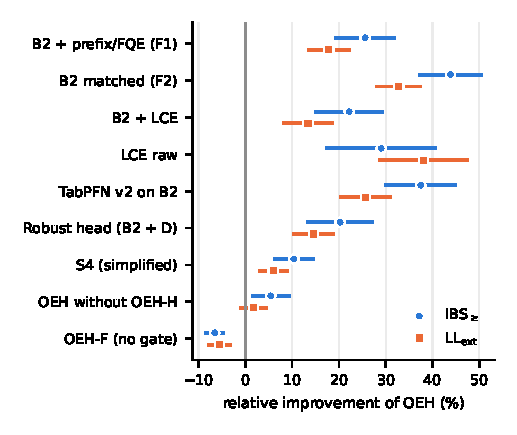
\includegraphics[width=\columnwidth]{figures/fig_panel6.pdf}
\caption{Test 3: relative improvement of \OEH{} over each comparator on the registered extrapolation endpoint, pooled over 192 MDPs; bars are 95\% MDP-cluster intervals of the absolute difference divided by the comparator's mean. The first two rows are the registered gates; the others are descriptive.}
\label{fig:panel6}
\end{figure}

\subsection{Is the gain retrospective?}
\label{sec:retro}
A forecaster could score well on $x1$--$x5$ by retrodicting what the pilot shows. On the opened panels, rescored post hoc on Eq.~\eqref{eq:ext}, the gain of \OEH{} over B2 on the extrapolation endpoint is at least as large as on the full endpoint in every scope (Test 1 external: 39.8\% $\mathrm{IBS}_\ge$, 26.2\% $\mathrm{LL}_{\rm ext}$; internal: 17.4\%, 11.2\%). The prefix/FQE baseline in its raw form is not competitive (LL 1.7--2.3 on 9 of 11 panels), but calibrated by the matched head it beats B2 by 18.4\% IBS on Test 1's external panels; \OEH{} still beats it there by 23.7\% IBS and 13.0\% LL. Test 3 then confirmed this ordering prospectively. Running the learner on the pilot is informative, but it is not enough.

\subsection{Where the gain comes from}
\label{sec:mechanism}
Fig.~\ref{fig:distance} pools the rows of Test 1 by shift distance. Near the training data ($d\le1.5$) the three predictors gain alike over B2; beyond $d_0=3$ the gate's combination beats both of its heads (at $d>4$: 0.32 nat for \OEH{}, 0.23 for the robust head, 0.11 for OEH-F), because it pairs the full head's censored probability with a finite law that transferred better there. Test 3 shows that this is not guaranteed. The distance sees only B2 statistics, so a change of logging behavior is invisible: SPIBB lies at $d\approx1.9$, and on the two SPIBB panels no method wins clearly. In the Murphy decomposition, \OEH{} and OEH-F gain mainly by \emph{resolution} outside the generator (Test 3: 0.12--0.13 against 0.06 for B2), not uniformly by calibration.

\begin{figure}[t]
\centering
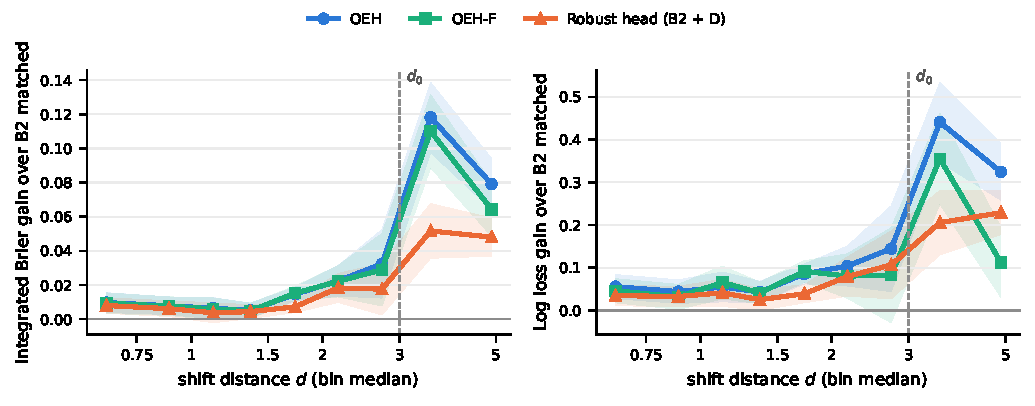
\includegraphics[width=\columnwidth]{figures/fig_gain_by_distance.pdf}
\caption{Gain over B2 by shift distance $d$ on Test 1 (rows pooled in nine bins; shaded: 95\% intervals; descriptive). The dashed line marks $d_0$.}
\label{fig:distance}
\end{figure}

\textbf{Features or learner?} TabPFN v2 on the 18 B2 statistics \emph{ties} \OEH{} inside the generator (\OEH{} is 1.9\% better in IBS and 0.7\% worse in LL, both intervals including zero), so most of the in-generator gain over B2 matched is reproduced by a stronger tabular learner on generic statistics. Outside the generator TabPFN only ties B2, and \OEH{} beats it by 37.4\% IBS and 19.5\% LL on Test 1 and by 31.4\% and 13.5\% on Test 3, where it was sealed before the labels. The value of the \OEH{} features lies in transfer.

\textbf{Components.} Inside the generator the information blocks are redundant: in a same-head leave-block-out on the opened cohort 7, removing any single block costs at most 1.4\% IBS. Outside it, rebuilding \OEH{} without OEH-H worsens Test 1's external IBS by $0.0028$ $[0.0012,0.0044]$ and Test 3's by $0.0048$ $[0.0023,0.0074]$, and without the direct posterior simulation worsens Test 1's external LL by $0.022$ $[0.011,0.033]$. Four simplified single-head candidates, specified with an acceptance rule before they were run, all failed it on 11 opened panels (the closest, S4, was 3.3\% worse outside and 8.0\% worse in IBS on Test 3). A nested leave-one-panel-out rerun of the whole gate selection puts its optimism at about one percentage point ($-5.6\%$ held-out vs $-6.6\%$ for one fit on all five panels, relative to OEH-F). These analyses are descriptive; no component claim is confirmatory.

\textbf{Label definition.} Rescoring the sealed forecasts on labels redefined with $\tau\in\{0.90,0.95,0.99\}$ and 7--9 of 10 seeds (reproducing all 11{,}988 official labels at $0.95$, 8/10), \OEH{} beats B2 outside the generator in all nine cells, but inside it is significantly \emph{worse} at $\tau=0.99$ (IBS $-8$ to $-10\%$): a forecaster fitted sharply for one target is penalized more when the target moves. On Test 3 the registered $\tau=0.99$ variant keeps the external ordering (\OEH{} .0964 / .989, B2 + prefix/FQE .1254 / 1.102, B2 .1554 / 1.233).

\subsection{Development evidence and negative results}
\label{sec:development}
Before the gate existed, OEH-F was tested on a sealed cohort of 84 generator MDPs: it lowered IBS by 15.97\% and LL by 10.22\% relative to B2, and all 22 registered contrasts, including two privileged ones, had positive simultaneous bounds. The gain was clear for CFQI and IQL, uncertain for BC (90.7\% censored) and absent for bottleneck MDPs. Table~\ref{tab:replication} lists the later development panels. On Colosseum, 77--98\% of the IBS gain came from censored rows and OEH-F's finite-budget law was worse than B2's: replacing it lowered OEH-F's LL from 0.890 to 0.856, which motivated the gate. Three earlier formulations failed their own sealed tests. On published BRIDGE MDPs~\cite{laidlaw2024stochastic}, with our pilots and labels, OEH-F was learner-dependent (better for CFQI, worse for IQL on Atari), and on the FourRooms offline log~\cite{farama_minari_fourrooms} the Dirichlet transition component lost to maximum likelihood.

\begin{table}[t]
\centering
\caption{Development panels of OEH-F (IBS / LL). LB: simultaneous lower bound of the improvement over B2.}
\label{tab:replication}
\footnotesize
\setlength{\tabcolsep}{2.2pt}
\resizebox{\columnwidth}{!}{%
\begin{tabular}{@{}lrcccc@{}}
\toprule
Panel & MDPs & OEH-F & B2 & LB vs B2 & vs robust head\\
\midrule
Cohort 7 (sealed) & 84 & .0460 / .563 & .0547 / .627 & $+.0027$ / $+.030$ & ---\\
Cohort 8 & 168 & .0466 / .548 & .0566 / .614 & $+.0066$ / $+.047$ & GO\\
Colosseum 2027 & 72 & .1010 / .890 & .1342 / .982 & $+.0151$ / $+.0003$ & NO-GO\\
Colosseum 2028 & 72 & .1050 / .895 & .1436 / 1.000 & $+.0176$ / $+.0060$ & NO-GO\\
SPIBB & 108 & .0192 / .366 & .0209 / .387 & $-.0005$ / $-.0060$ & ---\\
\bottomrule
\end{tabular}}
\end{table}

\subsection{Selection, cost and decision value}
\label{sec:cost}
\textbf{Selection.} A selector frozen before cohort 7's outcomes, using CFQI's pilot features, its OEH-F probabilities and the MDP-family label, chose among seven learners at $x10$. Against fixed CFQI it raised seed success by 6.67 points (LB $+4.26$) and normalized return by 0.0187 ($+0.0103$); against an earlier internal router the bounds crossed zero. \textbf{Cost.} Posterior simulation dominates \OEH{}'s cost (67\% of the pilot-input time on Test 1's internal panel; median 10.7\,s per MDP--behavior pair), grows quickly with $SA$ and exceeded our dense-model cap on most BRIDGE tasks; the gate adds no measurable cost. \textbf{Decision value.} Under the registered rule (collect the smallest budget whose forecast success probability reaches $q=0.8$, penalty $\kappa=100$), regret on Test 1 is 13.1 for \OEH{}, 15.1 for the robust head and 16.5 for B2 inside, and 20.0, 28.1 and 35.8 on forest; \OEH{} and OEH-F differ by at most 1.1 units on every panel. Theorem~\ref{thm:regret} and its variants hold on all four Test-1 panels but are loose (plug-in regret 4--36 units against bounds of 24--101). These figures exclude the cost of the pilot and of \OEH{}, so we make no claim of data or compute savings.

\textbf{Limitations.} All MDPs are tabular with $SA\le256$ and exact evaluation, and the label depends on a 0.95 threshold, ten seeds, an 8/10 sustained rule and a six-point grid. 71\% of meta-training rows are censored, and 91--98\% of censored rows in Test 1 still fail at $x200$. The posterior smooths the behavior and assigns zero reward to unobserved keys, which can mislead BC forecasts. The shift distance does not detect behavior shift, and adding behavior families to meta-training did not help. Inside the generator, a strong generic tabular learner matches \OEH{}.

\section{Conclusion}
\label{sec:conclusion}
From a pilot of a stochastic tabular MDP, \OEH{} forecasts the learner-specific, right-censored data requirement of BC, CFQI and IQL better than the same forecasting procedure on generic pilot statistics in three pre-registered tests on 660 new MDPs from the internal generator and seven external sources (in the registered comparisons of Tests 1 and 3, and descriptively in Test 2). On the last test, whose endpoint was restricted to the budgets the pilot cannot reach, it also beat a calibrated baseline that runs the learner on pilot prefixes and scores it by fitted Q evaluation. The evidence also delimits the method. The shift gate helped in two tests and hurt in the third; the advantage over the strongest pilot-only control was panel-dependent; a behavior shift that leaves the pilot statistics in range is invisible to the gate; and inside the generator a tabular foundation model on generic statistics matches \OEH{}, so the contribution of its features lies in transfer. The guarantees bound the gate's loss and link forecast scores to decision regret; they do not make \OEH{} consistent. Next steps are a shift measure for logging behavior, smaller pilots with measured net savings, and posteriors that scale beyond dense tabular models.


\section*{Reproducibility and data availability}
Every protocol, pre-outcome seal, prediction, label and analysis cited here is in the repository under \url{artifacts/}, indexed by \url{docs/week8/README.md}; the scripts named there regenerate every number and verify the sealed hashes. Raw pilot buffers and individual learner-job records are stored locally, so a public clone verifies the published artifacts but cannot rerun all learner jobs.

\bibliographystyle{IEEEtran}
\bibliography{references}
\end{document}
